\section{Lab4: Modulación ASK en GRC}

%*********************
\begin{frame}{}

\pgfdeclareimage[width=\paperwidth,height=\paperheight]{bg}{imagenes/fondocap2}
\setbeamertemplate{background}{\pgfuseimage{bg}}

\bfseries{\textrm{\LARGE Lab4\\ \Large Modulación ASK en GRC}}
\raggedright
\end{frame}
%*********************


\begin{frame}{Modulación ASK en GRC}

\pgfdeclareimage[width=\paperwidth,height=\paperheight]{bg}{imagenes/fondo3}
\setbeamertemplate{background}{\pgfuseimage{bg}}


\begin{figure}[H]
\centering
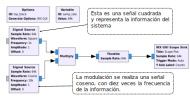
\includegraphics[width=\textwidth]{lab4/pdf/lab4_1.pdf}
\end{figure}
\end{frame}
%--------------------

\begin{frame}{Modulación ASK en GRC}
\begin{figure}[H]
\centering
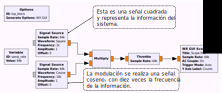
\includegraphics[width=\textwidth]{lab4/pdf/lab4_2.pdf}
\end{figure}
\end{frame}
%_---------------------

\begin{frame}{Modulación ASK en GRC}
\begin{figure}[H]
\centering
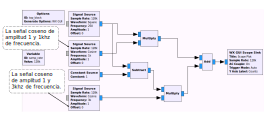
\includegraphics[width=\textwidth]{lab4/pdf/lab4_3.pdf}
\end{figure}
\end{frame}
%_---------------------

\begin{frame}{Modulación ASK en GRC}
\begin{figure}[H]
\centering
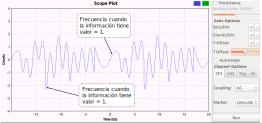
\includegraphics[width=\textwidth]{lab4/pdf/lab4_4.pdf}
\end{figure}
\end{frame}
%_---------------------

\begin{frame}{Modulación ASK en GRC}
\begin{figure}[H]
\centering
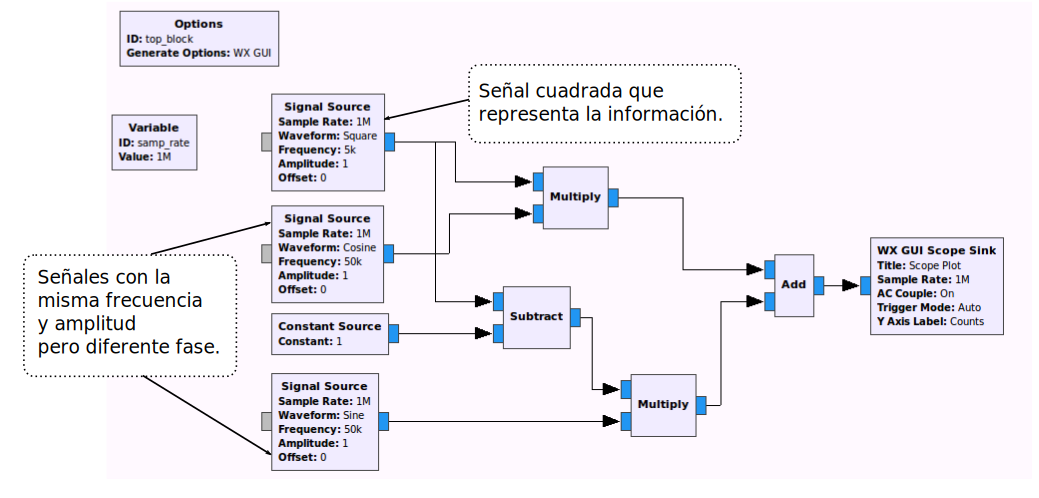
\includegraphics[width=\textwidth]{lab4/pdf/lab4_5.pdf}
\end{figure}
\end{frame}
%_---------------------

\begin{frame}{Modulación ASK en GRC}
\begin{figure}[H]
\centering
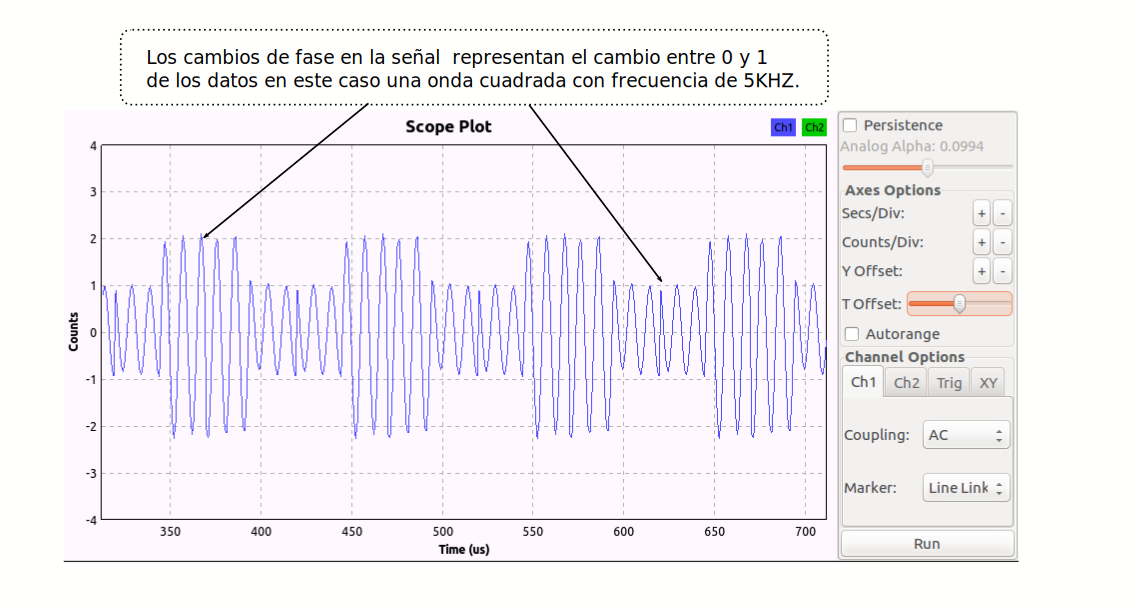
\includegraphics[width=\textwidth]{lab4/pdf/lab4_6.pdf}
\end{figure}
\end{frame}
%_---------------------